\section{eo\-Op$<$ EOType $>$ Class Template Reference}
\label{classeo_op}\index{eoOp@{eoOp}}
Abstract data types for {\bf EO}{\rm (p.\,\pageref{class_e_o})} operators.  


{\tt \#include $<$eo\-Op.h$>$}

Inheritance diagram for eo\-Op$<$ EOType $>$::\begin{figure}[H]
\begin{center}
\leavevmode
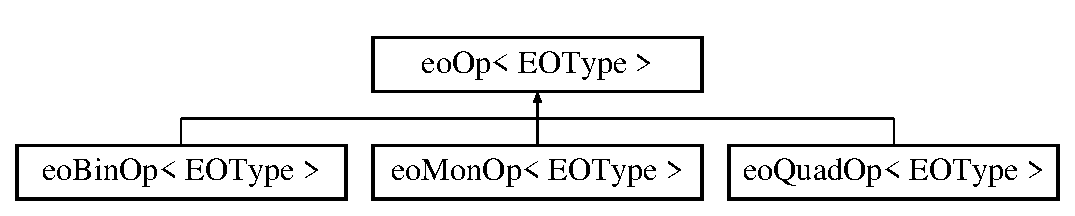
\includegraphics[height=2cm]{classeo_op}
\end{center}
\end{figure}
\subsection*{[NOHEADER]}
\begin{CompactItemize}
\item 
enum {\bf Op\-Type} \{ {\bf unary} =  0, 
{\bf binary} =  1, 
{\bf quadratic} =  2, 
{\bf general} =  3
 \}
\item 
{\bf eo\-Op} (Op\-Type \_\-type)\label{classeo_op_z14_1}

\begin{CompactList}\small\item\em Ctor. \item\end{CompactList}\item 
{\bf eo\-Op} (const {\bf eo\-Op} \&\_\-eop)\label{classeo_op_z14_2}

\begin{CompactList}\small\item\em Copy Ctor. \item\end{CompactList}\item 
virtual {\bf $\sim$eo\-Op} ()\label{classeo_op_z14_3}

\begin{CompactList}\small\item\em Needed virtual destructor. \item\end{CompactList}\item 
Op\-Type {\bf get\-Type} () const \label{classeo_op_z14_4}

\begin{CompactList}\small\item\em get\-Type: number of operands it takes and individuals it produces \item\end{CompactList}\item 
Op\-Type {\bf op\-Type}\label{classeo_op_z14_5}

\begin{CompactList}\small\item\em Op\-Type is the type of the operator: how many operands it takes and how many it produces. \item\end{CompactList}\end{CompactItemize}


\subsection{Detailed Description}
\subsubsection*{template$<$class EOType$>$ class eo\-Op$<$ EOType $>$}

Abstract data types for {\bf EO}{\rm (p.\,\pageref{class_e_o})} operators. 

Genetic operators act on chromosomes, changing them. The type to use them on is problem specific. If your genotype is a std::vector$<$bool$>$, there are operators that work specifically on std::vector$<$bool$>$, but you might also find that generic operators working on std::vector$<$T$>$ are what you need. 



Definition at line 68 of file eo\-Op.h.

The documentation for this class was generated from the following file:\begin{CompactItemize}
\item 
eo\-Op.h\end{CompactItemize}
